\documentclass[submission, copyright,creativecommons,sharealike,noncommercial]{eptcs}
\providecommand{\event}{Swarm community}
%
%
%%%%%%%%%%%%%%%%%%%%%%%%%%%%%%%%%%%%%%%
%%%%%%%%%% TITLE AND AUTHORS %%%%%%%%%%
%%%%%%%%%%%%%%%%%%%%%%%%%%%%%%%%%%%%%%%
\title{Liquid Democracy Voting System for the Swarm Platform}
\author{Fabrizio Romano Genovese
	\institute{Swarm Team}
	\institute{Quantum Group \\ University of Oxford}
	\email{fabrizio@swarm.fund}
\and
Jelle Herold
	\institute{Swarm Team}
	\email{jelle@swarm.fund}
}
\def\titlerunning{Voting System for the Swarm Platform}
\def\authorrunning{F.R.Genovese \& J. Herold}
\usepackage{wrapfig}
%
%
%%%%%%%%%%%%%%%%%%%%%%%%%%%%%%%%%%%%%%%
%%%%%%%%%%%%%% PACKAGES %%%%%%%%%%%%%%%
%%%%%%%%%%%%%%%%%%%%%%%%%%%%%%%%%%%%%%%
%% Display Graphics
\usepackage{graphicx}
%
%% Dynamic spacing for macros
\usepackage{xspace}
%
%% Define 'definition' environment
\usepackage{amsmath}
\usepackage{amsfonts}
\usepackage{thmtools}
\declaretheorem[
style=definition, 
name=Definition
]{definition}
%
%% Gothic letters to define the range set
\usepackage{eufrak}
%
%
%%%%%%%%%%%%%%%%%%%%%%%%%%%%%%%%%%%%%%%
%%%%%%%%%%%%%%% MACROS %%%%%%%%%%%%%%%%
%%%%%%%%%%%%%%%%%%%%%%%%%%%%%%%%%%%%%%%
%% Candidates and range sets
\newcommand{\candidates}{\ensuremath{\mathcal{C}} \xspace} 
\newcommand{\range}{\ensuremath{\mathfrak{R}}\xspace}
%
%% Contract names
\newcommand{\Candidates}{\textbf{CANDIDATES}\xspace} 
\newcommand{\Choices}{\textbf{CHOICES}\xspace} 
\newcommand{\Vote}{\textbf{VOTE}\xspace}
\newcommand{\History}{\textbf{HISTORY}\xspace} 
%%%%%%%%%%%%%%%%%%%%%%%%%%%%%%%%%%%%%%%
%%%%%%%%%%%%%%%%%%%%%%%%%%%%%%%%%%%%%%%
%%%%%%%%%%%%%%%%%%%%%%%%%%%%%%%%%%%%%%%
%\bibliographystyle{eptcs}
\PassOptionsToPackage{%
	backend=biber, %instead of bibtex
	natbib=true,% natbib compatibility mode (\citep and \citet still work)
	bibencoding=utf8,%
	language=auto,%
	style=numeric-comp,%
	sorting=nyt,% name, year, title
	backref=true,%"Cited on page..."
	firstinits=true%Only name initials
	%url=true
	%style=authoryear-comp, % Author 1999, 2010
	%bibstyle=authoryear,dashed=false, % dashed: substitute rep. author with ---
}{biblatex}
\usepackage{biblatex}
\addbibresource{Democracy.bib}
%
%
\begin{document}

%	\bibliographystyle{eptcs}
	
	\maketitle

	\begin{abstract}
		Here we highlight how the voting system is going to work. We will start briefly reviewing existent solutions, we will proceed sketching the general idea for the voting system on the Swarm Platform and, finally, we will dive into details producing a working algorithm.
	\end{abstract}

\section{Pre-existent solutions}\label{sec:Pre-existent solutions}
	The need to define a voting system is not a new problem for the blockchain community. For instance, if some altcoin is going to hard fork, the developing team will often ask the user base to express a preference about which branch to adopt. It is obvious, then, that in a situation like this some kind of procedure has to be devised to allow people to express this preference, that is, to allow people to vote.
	
	One of the most common ways to deal with this problem is by issuing some voting tokens and creating two addresses that stand for \emph{yes} and \emph{no}. Every user receives a number of tokens equal to the number of coins owned and sends them to one of these two addresses, expressing a preference.
	
	Albeit very simple to implement, this method has many fundamental flaws that make it not suitable for a system that has democracy -- and hence voting -- at its center:
	\begin{enumerate}	
		\item First of all, a voting procedure like the one highlighted above is very similar to majority voting and, as such, it is cursed by many downsides. One of the biggest achievement of social choice theory is proving that nearly all the voting systems that people intuitively consider ``fair'' are not fair at all, meaning that they are prone to any sort of manipulation or can even be dictatorial~\cite{Arrow1951, Satterthwaite1975, Gibbard1973}. Voting with tokens as stated above is no exception. 
		%
		\item In the very same moment someone votes, the tokens are transferred to the address expressing a preference, and can be publicly seen. This means that a sufficiently skilled user is able to see in real time who is winning the vote. This exposes the system because gives away data that can be employed for any kind of manipulation.
		%
		\item ``Real'' tokens can be exchanged while the voting ones remain in one's wallet. This means that voting power is not really related to the quantity of money one owns: In a transaction happening after the voting tokens are issued, the person receiving the real tokens has no voting power whatsoever while, on the other hand, the other person retains the voting power without having real stake.
		
		For instance, someone with a lot of real tokens could sell them all, and then use the voting tokens he retained to vote for a very bad decision for the platform. At this point the tokens he just sold will be depreciated because of this bad decision and the person will be able to buy them back at a fraction of the price, making a profit. 
		
		This means that a very powerful user on the platform could exploit the democratic infrastructure to make direct profits.
		%
		\item There is no reputation system. This means that a user voting power is only proportional to the amount of coins owned. A lot of important parameters (how active that user is on the platform, how much money one moves every month, how much that user helped with proposals, \dots) are completely disregarded.
		%
		\item Vote delegation is messy, or even not impossible.
	\end{enumerate}
%
	For these reasons we deemed necessary to steer away from all the pre-existing solutions and design an ad-hoc voting environment that is reasonably fair (according to social choice theory) and suitable to be used on a daily basis.
%
%
\section{Range Voting}\label{sec:Range voting}
	\begin{wrapfigure}{r}{0.5\textwidth}
		\vspace{-10pt}
		\begin{center}
			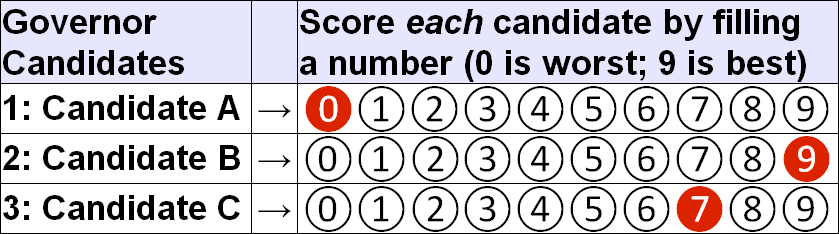
\includegraphics[width=0.48\textwidth]{Voting_Ballot.png}
		\end{center}
		\vspace{-15pt}
		\caption{Range voting ballot [source: Wikipedia]}\label{fig:Ballot}
		\vspace{-5pt}
	\end{wrapfigure}
%
	The voting method we choose for the platform is \emph{range voting}. Range voting is one of the fairest voting systems available. In particular, being it a \emph{cardinal} and not an \emph{ordinal}\footnote{These are technical terms of voting theory. You can safely ignore them if you don't know what they mean.} voting system, many of the mathematical results about unfairness and dictatorship, such as~\cite{Arrow1951, Satterthwaite1975}, do not apply.
	
	In range voting, each voter can rank each choice giving a score, for instance from $0$ to $9$, where $0$ stands for ``I absolutely don't like this choice'' and $9$ stands for ``I absolutely love it'' (see for instance Figure\ref{fig:Ballot}). When the voting closes, the scores for each choice are summed, and the choice with more points is the one that wins.
	
	There are many groups that actively advocate for range voting to be adopted in electoral laws all around the world, and in addition to this range voting is also considerd one of the best voting procedure available in company administration (see, for instance~\cite{Electology, RangeVoting}). 
	
	To conclude, in choosing the right voting procedure for the Swarm platform we consulted decades of research and study on voting systems to find the best alternative available, and we are fairly convinced that range voting is the one.
%
%	
\subsection{Reputation}\label{subsec:Reputation}
%
	Taking into account ``modifiers of the voting power'' is also very easy when one adopts range voting. Let's suppose, for instance, that we want to have a system where the power of a voter is proportional to the number of coins he owns. If voter $A$ owns $n$ coins, then it will be sufficient to multiply by $n$ all the scores that $A$ gives to each candidate. So, for instance, if $A$ owns $10$ coins and ranks a candidate with a score of $5$, that candidate will receive $10*5=50$ points.
	
	To be precise, we want to take into account more parameters than just the quantity of money a voter has to determine the voting power, but now we do not need any new concept to do this. For each user $A$, we will just calculate a multiplier, denoted with $\rho_A$ and called \emph{reputation of $A$}, considering all the parameters that we deem relevant. Again, everything we will need to do to make $A$'s votes proportional to his reputation is to multiply all the scores that $A$ assigns by $\rho_A$.
%
%
\subsection{Drafts}\label{subsec:Drafts}
%
	Clearly, it may happen that a vote leads to a draft. In range voting this means that there are two or more candidates at the top of the points list having the same score. For instance, imagine we have to elect three people for a company board and there are ten candidates, with their ranking in terms of points as follows:
	\begin{center}
	\begin{tabular}{| l | r |}
		\hline
		\textbf{Candidate} & \textbf{Points}\\
		\hline			
		Candidate 7 & 247\\
		Candidate 2 & 133\\
		Candidate 5 & 102\\
		Candidate 8 & 102\\
		Candidate 10 & 84\\
		Candidate 1 & 58\\
		Candidate 6 & 37\\
		Candidate 3 & 29\\
		Candidate 9 & 14\\
		Candidate 4 & 3\\
		\hline  
	\end{tabular}
	\end{center}
%
	Since we are selecting only three members for the board, we have to pick the three best performing candidates. This obviously includes candidates $7$ and $2$, but then we are stucked because candidate $5$ and $8$ have the same amount of points. So who who among the two do we choose?
	
	In classic range voting, at this point, another voting round is held. We discussed at length about implementing such a system for Swarm, and we decided that it wasn't a good idea, first because it puts much more stress and responsibility on users that will have to vote two times, and second because it would make the actual code much more complicated and difficult to audit. So we went for a system in which no second round is needed, as follows:
	\begin{itemize}
		\item If there is an ex-aequo situation, we will prefer the candidate with the highest reputation.
		\item If this doesn't solve the problem (there are multiple winning candidates with the same reputation), then the choice is pseudorandom.
	\end{itemize}
%
%
\section{The voting algorithm -- Intuitive explanation}\label{sec:Voting intuitive}
%
\subsubsection{Desiderata}\label{subsubsec:Desiderata}
	Now that we know what we want, we have to implement it. There are some fundamental desiderata we require:
	\begin{itemize}
		\item The voting should be transparent. This means that all the relevant information should be stored on the blockchain, and every user should be able to calculate the vote outcome independently, as well as to check that is preference was correctly submitted.
		%
		\item The voting should be encrypted. As we said in Section~\ref{sec:Pre-existent solutions}, one problem of voting on the blockchain is that people can know who is winning before the voting window closes. To avoid such a situation, every vote should be encrypted and readable only when the voting window closes.
		%
		\item Being an active member of the Swarm democracy should increase a member reputation. Swarm values participation, and it makes sense that ``the more you vote, the more your vote becomes powerful''. This is also a way to value the experience and time spent on the platform.
		%
		\item The reputation should also be proportional to the amount of Swarm tokens owned. More specifically, if one owns zero Swarm tokens then his voting power should be zero (meaning that has no influence whatsoever).
		%
		\item Delegation must be possible. The word ``delegation'' is actually the reason why we talk about \emph{liquid democracy} and not just about \emph{deocracy}. The idea here is that any Swarm member can delegate some other member to vote in his place. This is particularly useful when someone is asked to take a decision, but does not feel to have enough experience or understanding to vote. Instead of wasting his preference, in such situation a user can delegate someone else to vote in his place.
		Imagine, for instance, that Bob is a Swarm user. Bob has to vote to elect members of the administration Board. He reads all the proposals and what every member wants to do, but it is all incredibly technical and out of his skill set. Bob, on the other hand, knows that Alice, a professional trader which he trusts, is on Swarm too. What Bob can do is delegating Alice to vote for him, so that his preference will not be wasted.		
	\end{itemize}
%
%
\subsubsection{User experience}\label{subsubsec:User experience}
%
	From the point of view of a Swarm user, voting should be simple. The idea is that you just visit a webpage, and use the ethereum address you have your tokens on as a login. At this point, you are able to see your reputation and all the open voting windows. To vote, it is sufficient to rank each candidate on the webpage and sign your preference with your private key. At this point, the preference is submitted. To improve easy of use, we are working to make such webpage compatible with Nano Ledger S and Trezor, so that signing your petition will just require a couple of clicks.
	
	When the voting window closes and the outcome is calculated, the user should will be able to see it on the very same web page.
%
%
\subsubsection{Voting phases}\label{subsubsec:Voting phases}
%
	There are two different kinds of votes on Swarm. The first kind is when the user base has to express a preference. The board may ask, for instance, ``Do you prefer option A or option B?'' and in this case everything that is needed is voting. 
	
	The second kind is when the vote is about electing people to occupy a position, for instance when the user base has to elect members for the Swarm board. In this case, we have to implement a ``campaign phase'' before the vote itself, where people are actually able to propose themselves for the position.
	
	What we want then is as follows:
	\begin{itemize}
		\item A phase I (optional, depending on the kind of vote) to manage candidatures.
		\item A phase II that is the vote itself.
	\end{itemize}
%
%
\subsection{The Voting Algorithm}\label{subsec:Intuitive algorithm explanation}
%
\subsubsection{Phase I}\label{subsubsec:Intuitive Phase I}
	During phase I (if the kind of vote comprises it), users will have a time window to propose themselves for the election. This is what happens:
	\begin{itemize}
		\item Phase I time window opens. A smart contract called \Candidates is created. It will contain information about all the candidates running for the election.
		%
		\item Any user, logging in with his ethereum address, can see this on the webpage. He can, if he wishes to, decide to run for the election. To do this the user has to fill a couple of fields: One is a ``bio'' field where the user says something about himself. The other is a ``letter of intent'' where the user states why he wants to run for the election. The candidature can be submitted signing it with the user private key.
		%
		\item Every time a candidature is submitted, the \Candidates contract checks that no other candidature has been already submitted by that ethereum address. This is because, obviously, one user can run only once for the same vote, and also to prevent spamming. If this is the case, the candidate is not added to \Candidates and the submission is rejected with an error message. Otherwise, it is.
		%
		\item When the Phase I time window closes, it is not possible to add further candidates to \Candidates.
	\end{itemize}
%
%
\subsubsection{Phase II}\label{subsubsec:Intuitive Phase II}
%
	During Phase II the actual voting happens, as follows:
	\begin{itemize}
		\item Phase II voting window opens. A smart contract called \Vote is created. It will contain information about all the candidates running for the election.
		%
		\item A Swarm trusted party\footnote{The Estonian non-profit, for instance} creates a couple of public/private keys. The private key is kept secret, while the public key is pushed into the \Vote contract.
		%
		\item Every user can see the open vote on the web page, with all the set of choices/candidates to rate. If Phase I was present, the set of candidates is automatically derived from the \Candidates smart contract. 
		%
		\item The user can vote as follows: He can rank each candidate giving him a score (from $-3$ to $3$, the default being $0$). He can moreover specify an ethereum address to delegate his vote to someone else. 
		
		Note that these two things are not mutually excluding: If for some reason the delegation shouldn't work (for instance if your delegate forgets to vote), then the algorithm will immediately fall back on the scores the user gave. It makes sense then that you express a vote even when you specify a delegate to vote for you.
		%
		\item When the user pushes the ``submit'' button, all his voting preferences and delegate addresses are encrypted using the public key found in \Vote. The user is then prompted to sign his submission with his private key, as usual.
		%
		\item When the Phase II voting window closes, it is not possible to push more voting preferences to \Vote.
	\end{itemize}
%
%
\subsubsection{Outcome}\label{subsubsec:Intuitive Outcome}
%
		The outcome of the vote is then calculated, as follows:
		\begin{itemize}	
			\item Shortly after the Phase voting window closes, the Swarm trusted party appends the secret key that was generated in the previous phase to \Vote. At this point, all the information contained in \Vote becomes accessible to everyone.
			%
			\item \Vote is decripted, and the outcome is calculated offline. This is still trustable since every user can repeat this procedure on his own computer (this functionality will be provided on the web page, and every user will be able to check that the outcome was calculated correctly with client-side).
			%
			\item First of all, the algorithm check for repeated votes, that is, users that submitted their vote more than once. This being the case, the algorithm just cancels all the submitted votes but the most recent one.
			%
			\item After this, the algorithm checks that no vote comes from the Swarm foundation address, and this being the case, cancels that voting preference from the contract. This is for ethical reasons. In fact, Swarm founders could use the Swarm foundation to express a vote. Since the Swarm foundation holds 33\% of the total Swarm tokens, its would be so high to turn Swarm into a dictatorship. Swarm team members and partners are obviously still able to vote using their personal wallets, as any other member.
			%
			\item The algorithm pushes information into the \History contract, that registers how many times a user expressed a vote. This paramenter is used to calculate the reputation of a user, since it representative of the user activity and contribution to the platform
			%
			\item The algorithm solves delegation errors. In fact, it may be that a user called Bob delegated Alice to vote for him, but Alice forgot to vote. It could also be that Bob delegated Alice, Alice delegated Charlie and Charlie delegated Bob. As you can see, this is a loop and it is difficult to say who is deciding for who. The algorithm addresses this situation falling back to the personal preferences. For instance, if Bob delegated Alice and Alice forgot to vote, then the algorithm uses the scores that Bob gave. In the worst case, Bob left everything as it was, meaning that he had scored $0$ every candidate.
			%
			\item The algorithm calculates the reputation of every voter. To do this, it checks how many tokens the voter holds, checks if there are more reputation modifiers referring to that user in the \History contract, and puts everything together. At this point two things can happen:
			\begin{itemize}
				\item If the user voted for himself, the algorithm multiplies the scores that the user gave by his reputation.
				
				\item If the user delegated someone else, the algorithm transfers the user reputation to that someone to calculate the scores.
			\end{itemize}
			%
			\item Finally, the algorithm calculates the winning choice/candidate summing all the scores together. As we pointed out in Section~\ref{sec:Range voting}, if there are ex-aequo candidates then the algorithm checks who has the bigger reputation to calculate the winner\footnote{Note that if the voting is about choices and not candidates, this is not possible since choices do not correspond to single users and hence have no reputation. In this case this step is just skipped}. If this is not enough, the algorithm chooses between the winning alternatives pseudorandomly.
			
			Should be this the case, the user will receive a notification warning him: Since the final choice is pseudorandom, clearly the outcome calculated in locale may be different from the outcome calculated by Swarm team.
			
			\item The Swarm team publishes the result of the vote, that is displayed in the user web page. As we said, the user can independently check that the outcome has been calculated correctly.
		\end{itemize}
%
%
\section{The Algorithm, detailed explanation}\label{sec:Algorithm technical explanation}
%
	\textbf{Note:} This section is technical and requires some basic familiarity with mathematics and coding. The following algorithms are not even written as pseudocode, and use evil instructions like ``goto''. This choice has been made to improve readability and give an idea of what are the actions that the algorithm has to perform. The real modules used will be most likely coded using functional programming. Please refer to our github repo to check the actual source code.
%
%
\subsection{Definitions}\label{subsec:Definitions}
%
	\begin{definition}
		A \emph{string} $s$ is a finite sequence of characters or digits $s_1 s_2 \cdots s_n$. If $s$ is a string, we will denote with $s[n]$ the \emph{n-th} character of $s$, and with $|s|$ the \emph{length} of $s$. We will abuse this notation and we will often use \emph{strings of strings}, that is, some string $s$ such that $s[n]$, for some $n$, is a string too. In this case, we will denote with $s[n][m]$ the $m$-th entry of the $n$-th entry of $s$.
		
		If $s$ is a string of numbers and $k$ is a number as well, then $k*s$ is the string $(ks[1], \dots, ks[|s|])$.
	\end{definition}	
%	
	\begin{definition}\label{def:candidates and range}
		We will denote with \candidates the \emph{ordered} set of candidates or choices that can be voted for in a given vote. We will denote with \range the set of possible scores a user can assign to each candidate. For instance, if we have three possible choices $A,B,C$ and the range of possible scores goes from $-3$ to $3$, then $\candidates := \{A, B, C\}$ and $\range := \{-3,-2,-1,0,1,2,3\}$. We will moreover denote with $| \candidates|$ and $|\range|$ the number of elements that these two sets have. In our example, $|\candidates | = 3$ and $|\range|=7$.
	\end{definition}
%	
	\begin{definition}\label{def:voting string}		
		We can express the voting of a user as a string $(a,b,c, \dots)$, where $a,b,c \in \range$. $a$ represents the rating given to candidate $A$, $b$ the rating given to candidate $B$ and $c$ the rating given to candidate $C$ and so on. This string is called \emph{preference string}, and its length is clearly equal to $|\candidates|$.
	\end{definition}
%
	\begin{definition}
 		We denote an user $A$ delegating his/her vote to a user $B$ with $A \to B$.
	\end{definition}
%
%
\subsection{Contracts}\label{subsec:Contracts}
%
Here we highlight the fundamental pieces of information that will be specified in the three contracts we mentioned in Section~\ref{subsec:Intuitive algorithm explanation}.
\subsubsection{The \Candidates contract}
	In every \Candidates contract, there will be a reference to the correspondent \Vote contract, on which the preferences of the users will be registered. This piece of information is specified when the contract is created and allows the user to reconstruct where he has to send his preferences once the voting window opens.
	
	The data in the \Candidates contract is list of strings that look like this: 
	\[
		c := (\text{candidate ethereum address} \mid \text{hash of the bio} \mid \text{hash of the statement of purpose})
	\]
	%
	Every time some candidate pushes his candidature string $c$ to the chain, it is appended to this list. 
	
	\Candidates does not do any special computation, aside of the following:
	\begin{itemize}
		\item If $c$ is pushed to \Candidates, check the status of the time window.
		\item If the time window is closed, reject $c$.
		\item Check that $c[1]$ corresponds to the same address that is trying to append the string. If not, someone is running with a fraudulent address, and $c$ is rejected.
		\item Otherwise, check if there is some $c'$ such that $c'[1] = c[1]$.
		\item If this is the case, $c'$ is deleted and $c$ is added at the bottom of the contract (this allows a candidate to modify his statement of purpose or bio until the window stays open).
	\end{itemize}
%
	This means that we avoid double candidatures, make sure that the candidatures are not fraudulent and allow any candidate to modify his bio/statement of purpose until the time window stays open.

	The $c[2]$ and $c[3]$ fields of the string guarantee that the candidate bio and statement of purpose are not altered. They can now be stored on an independent server minimizing the space consumed and still guaranteeing that the platform system stays trusted.	 
%
%
\subsubsection{The \Choices contract}
	As we mentioned, there are two kind of votes on the Swarm platform. The first kind allows for a Phase I where people can propose themselves as candidates, while the second does not, giving people the possibility to express a preference in a set of pre-determined choices (this is the case for a typical ``yes/no'' voting, for instance).
	
	The \Candidates contract addresses the voting of the first kind, allowing users to add their candidature in it. The \Choices contract is used for the votes of the second kind, and contains the set of choices the users will be able to vote. 
	
	Note that since a vote can have or not have a Phase I, these two contract are \emph{mutually eclusive}: A voting relies on a \Candidates contract or on a \Choices contract, but not on both at the same time.
	
	As in the previous case, in every \Choices contract there will be a reference to the correspondent \Vote contract, on which the preferences of the users will be registered. This piece of information is specified when the contract is created and allows the user to reconstruct where he has to send his preferences once the voting window opens.
	
	The data in the \Choices contract is a list of strings that look like this: 
	\[
	c := (\text{choice} \mid \text{hash of the choice description})
	\]
	%
	$c[1]$ represents the kind of choice we are going to vote (``yes'' or ``no'', for instance), while $c[2]$ is the hash of a description of what that choice means (for instance ``Voting this you are approving the following board resolution: \dots"). 

	This contract doesn't perform any computation whatsoever.
	
	The $c[2]$ field of the string guarantees that the description of a given choice can be stored on an independent server minimizing the space consumed and still guaranteeing that the platform system stays trusted.	 
%
%
\subsubsection{The \Vote contract}
	The data in the \Vote contract is of different kinds, as follows:
	\begin{description}
		\item[Secret key:] This is specified in the contract when it is created. It is a RSA (or similar) secret key, denoted with \emph{pub} and generated by a Swarm trusted party.
			
		\item[Instructions:] These are again specified when the contract is created, and are used to calculate the voting outcome. They consist of two parameters: an integer, representing the number of choices that have to be declared as winners (for instance, ``the three best candidates have to be picked''), and the range of possible values used for range voting, denoted with $\range$ (for instance $\{-3,-2,-1,0,1,2,3\}$\footnote{By definition, we require $0$ to be always present in the range, and the range to be symmetric, meaning that the values can go from $-x$ to $x$, for some integer $x$.}).
		%
		\item[Encrypted block:] This is a list of encrypted strings, that look like this when decrypted:
		\[
		v := (\text{user address} \mid \text{preference string} \mid \text{delegation address})
		\]
		Such strings are called \emph{voting strings}, and have following specification:
		\begin{description}
			\item[user wallet address] is the ethereum address of the voter;
			%
			\item[preference string] is a string defined as in Definition~\ref{def:voting string}, where $\candidates$ (see Definition~\ref{def:candidates and range}) is the set of all the addresses in \Candidates. To be specific, the first entry of the voting string refers to the first candidate in \Candidates, the second to the second candidate in \Candidates and so on.
			%
			\item[delegation address] is an eth address.
		\end{description}
		When the voting window opens, every user can encrypt his voting string with \emph{pub} and add it to the encrypted block.
		%	
		Note that since these stings will be added in an encrypted form, their integrity can't be checked by the contract itself, and will have to be verified offline (see module~\ref{subsubsec:Check that every string is well formed}).
		
		When the voting window closes, the users will not be able to add more strings to the contract. The list of all the encrypted strings as above will be called \emph{encrypted block}.
		
		\item[Secret key:] This is added to the contract by the same trusted party that generated \emph{pub} after the voting window closes. This secret key, denoted with \emph{sec}, allows to decrypt the encripted block.
		
		\item[Plain block:] This is just the encrypted block itself, decrypted with \emph{sec} and purged of incorrect specifications and delegation loops, according to module~\ref{subsubsec:Get plain block}. It will be added to the contract by a Swarm tusted party after the voting window closes.
			
		\item[Winner:] The list of winner(s) of the election, again added to the contract by a Swarm trusted party when the voting window closes. This is just a list of numbers bigger or equal to $1$, referencing to the \Candidates or \Choices contract. If this list is, for instance, $(3,6,2)$, this means that the 3\textsuperscript{rd}, the 6\textsuperscript{th} and the 2\textsuperscript{nd} candidate (choice) listed on \Candidates (\Choices) are the ones who won. 
		
		To get the corresponding winning candidate (choice) value it is sufficient to fetch the first value of the string in the contract. For instance, in the previous example, if our contract is of type \Candidates then the winning ethereum addresses are ``3\textsuperscript{rd} listed string''[1], ``6\textsuperscript{th} listed string''[1] and ``2\textsuperscript{nd} listed string''[1].

	\end{description}
	This contract is very simple. It is just a big database, with an encrypted and a plain text part. The only real computation that the database does is checking if the user can or cannot add a voting string to it verifying if the voting window is open or not and, in a latter stage, authorizing only the Swarm trusted party to add information to it.

	\textbf{Note}: On the user web page, before any preference is specified, vote strings and delegation addresses are set to the defaults values of $0$ for $v[3]$ and $(0,0, \dots, 0)$ for $v[2]$. In this way, if the user submits his vote without specifying any preference, its vote will still be submitted as well formatted.
		
	\textbf{Note}: The reason why the plain block is added to the contract is to make the outcome verification process faster. On the user web page, in fact, the user will have the possibility to check independently the outcome of a vote. To do this, some code will be run client-side. The user will be able to select between three modes:
	\begin{itemize}
		\item A ``thorough'' mode that obtains the plain block applying module~\ref{subsubsec:Get decrypted block}, verifies that this coincides with the plain block added to \Vote by the Swarm trusted party and then calculates the vote outcome, that is again compared with the list of winners attached to \Vote. With this option nearly every step of the calculation is executed locally.
		
		\item A ``fast'' option that skips the first part, and just uses the plain block provided on the \Vote contract to calculate the outcome. This will undoubtably be faster, since all the decryption and purging will be skipped.
		
		\item A ``paranoid'' option that works as the ``thorough'', with the exception that now module~\ref{subsubsec:Get reputation for every user} does not use the plain block of previous contracts to calculate reputations, but invokes module~\ref{subsubsec:Get decrypted block} every time. This will require \textbf{a lot} of decryption and purging, and will probably be very very slow to run. On the other hand, here \textbf{every} step of the calculation is executed locally, and nothing is given for granted.
	\end{itemize} 
%
%
\subsubsection{The \History contract}\label{subsubsec:The reputation contract}
	The data in the \History contract is just a list of references to all the \Candidates and \Choices contracts produced. 
	
	Every time a new voting is open, a new \Candidates (only if the vote has a phase I) or \Choices contract is produced. A Swarm trusted party adds a reference to these contracts to \History. 
	
	This contract is useful for two reasons:
	\begin{itemize}
		\item Since both \Candidates and \Choices contracts always contain a reference to their corresponding \Vote contract, every user is able to follow the references to see how many votes and candidatures an address submitted. This information is used to calculate the reputation of a user by module~\ref{subsubsec:Get reputation for every user}.
		
		\item The \History contract is also used by the user web page to fetch the history of all the votes performed by the platform. Following the references any client can display which votes have been performed and for which ones Phase I and Phase II time windows are still open.
	\end{itemize}
%
%	
\subsection{Modules}\label{subsec:Modules}
%	
	Here we formalize some algorithms that will perform various operations to get a vote outcome, such as getting rid of delegation loops. These algorithms will be invoked to perform the voting, both locally and by the Swarm trusted party.
	
\subsubsection{Display votes}\label{subsubsec:Display votes}
	This algorithm is used to display all the votes that happened on the platform, including the open ones. It is used in particular in the front end environment.
	\begin{itemize}
		\item Scroll the \History contract and follow the references, building a history of voting contracts. Every reference also gives the relevant time window for a given contract, that then can be displayed as open or closed on the user web page.
		
		\item When the user clicks on a given vote, fetch from an independent server all the relevant information. Verify that the hashes are correct on the correspondent \Candidates or \Choices contract.
		
		\item At this point, depending on the time window, a user will be able to vote, run for an election or verify the outcome of a vote. Again, Following the reference on the corresponding \Candidates and \Choices contracts, the user will be able to know which \Vote contract has to be consulted to manipulate this information.
		
		\item For instance, if a user wants to verify the outcome of a vote, he follows the unique identifier in the corresponding \Candidates (\Choices) contract and applies module~\ref{subsubsec:Calculate vote outcome} to this. If the final result corresponds to the winner(s) displayed in \Vote, well. Otherwise, display an error.
	\end{itemize}

\subsubsection{Submit candidature}\label{subsubsec:submit candidature}
	This is the algorithm to submit a candidature for a vote.
	\begin{itemize}
		\item Check if the time window allows you to submit your candidature to \Candidates. If not, return with an error.
		\item Calculate the hash of the ``bio'' form, call it \emph{bio}.
		\item Calculate the hash of the ``statement of purpose'' form, call it \emph{statement}.
		\item Upload these two forms on the independent server.
		\item Form the string $c:= (\text{your ethwallet} \mid \emph{bio} \mid \emph{statement})$
		\item Add it to \Candidates signing with your private key.	
	\end{itemize}

\subsubsection{Submit vote}\label{subsubsec:submit vote}
	This is the algorithm to submit a vote.
	\begin{itemize}
		\item Check if the time window allows you to submit your vote to \Vote. If not, return with an error.
		\item Form the string $v:= (\text{your ethwallet} | \text{preference string} \mid \text{delegation address})$
		\item Fetch the public key \emph{pub} from $\Vote$. 
		\item Encrypt $v$ with $\emph{pub}$.
		\item Add it to \Vote signing with your private key.	
	\end{itemize}
		
\subsubsection{Get decrypted block}\label{subsubsec:Get decrypted block}
	This is the algorithm to decrypt the encrypted block in a \Vote contract and purge it by any kind of error.
	\begin{itemize}
		\item Use the secret key in \Vote to decrypt the encrypted block. Get a list of decrypted entries called \Vote' back. (module~\ref{subsubsec:Decrypt block}).
		\item Check that every string in \Vote' is well-formed (module~\ref{subsubsec:Check that every string is well formed}).
		\item Ban the Swarm foundation address (module~\ref{subsubsec:Ban foundation address}).
		\item Delete repeated votes (module~\ref{subsubsec:Delete repeated votes}).
		\item Get rid of hanging delegations (module~\ref{subsubsec:Get rid of hanging delegations}).
		\item Get rid of delegation loops (module~\ref{subsubsec:Get rid of delegation loops}).
		\item Return \Vote'.
	\end{itemize}


\subsubsection{Check vote outcome}\label{subsubsec:Calculate vote outcome}
This module verifies that the outcome of a vote is the one provided by the Swarm trusted party. 

First of all, fetch the number of winner(s) from the instructions of the $\Vote$ contract. Fetch the number of candidates (choices) from the \Candidates (\Choices) contract, call it $|\candidates|$. If $|\candidates| \leq w$, declare everyone a winner. Otherwise: 
	\begin{description}
		\item[Fast mode:] This is the fastest mode available. 
			\begin{itemize}
				\item Read the plain block from \Vote. Copy it to a local file \Vote'.
				\item Assign reputation to every user (module~\ref{subsubsec:Assign reputation to every user}, \textbf{fast} option enabled).
				\item Calculate the winner(s) (module~\ref{subsubsec:Get winner}).
			\end{itemize}	
		\item[Thorough mode:] This mode will be slower, but the only thing that won't be entirely checked are user reputations.
			\begin{itemize}
				\item Apply module~\ref{subsubsec:Get decrypted block} to \Vote.
				\item Read the plain block from \Vote. Check that the two coincide. If not, display an error.
				\item Assign reputation to every user (module~\ref{subsubsec:Assign reputation to every user}, \textbf{fast} option enabled).
				\item Calculate the winner(s) (module~\ref{subsubsec:Get winner}).
			\end{itemize}			
		\item[Paranoid mode:] This mode will be painfully slow, but will check everything locally.
			\begin{itemize}
				\item Apply module~\ref{subsubsec:Get decrypted block} to \Vote.
				\item Read the plain block from \Vote. Check that the two coincide. If not, display an error.
				\item Assign reputation to every user (module~\ref{subsubsec:Assign reputation to every user}, \textbf{slow} option enabled. This will take time).
				\item Calculate the winner(s) (module~\ref{subsubsec:Get winner}).
			\end{itemize}			
	\end{description}
Finally, check that the output result coincides with the one in $\Vote$ (module~\ref{subsubsec:Final check}).

\subsubsection{Decrypt block}\label{subsubsec:Decrypt block}
This module just uses the the secret key \emph{sec} in \Vote to decrypt the encrypted block.
	\begin{itemize}
		\item Fetch \emph{sec} from \Vote.
		\item Fetch the encrypted block from \Vote. Copy it to a file \Vote'.
		\item Denote with $\Vote'[n]$ each entry in \Vote'. Decrypt it:
		\begin{itemize}
			\item If $\Vote'[n]$ doesn't decrypt for some $n$ (probably it has been encrypted with the wrong public key), delete it.
			\item Otherwise, replace $\Vote'[n]$ with its decrypted version.
			\item Return \Vote'.
		\end{itemize}
	\end{itemize}


\subsubsection{Check that every string is well formed}\label{subsubsec:Check that every string is well formed}
	This algorithm checks that every voting string in \Vote' is in the right form.
	\begin{itemize}
		\item For every $n$, consider $\Vote'[n][1]$. Check that this is a valid ethereum address.
		
		\item Next, check that $\Vote[n]$ was pushed to \Vote by $\Vote'[n][1]$. This not being the case, it means that some ethereum address added a vote to $\Vote$ using a false identity. This being the case, erase the line $\Vote'[n]$. 
		
		\item Then, check how many candidates (choices) are in \Candidates (\Choices). This will be equal to the number of candidate (choice) strings present there. To keep consistent with our notation, denote this number with $|\candidates|$. Fetch moreover the range parameter $\range$ from \Vote. Check that, for every $n$, $\Vote[n][2]$ is a string of integers of length $|\candidates|$ with values ranging in $\range$. If this is not the case, again delete $\Vote[n][2]$.
		
		\item Finally, for every $n$, check that $\Vote'[n][3]$ is a valid ethereum address, or $0$. Again, if this is not the case, delete $\Vote[n][2]$.
		
		\item Return \Vote'.
	\end{itemize}
	
	
\subsubsection{Ban foundation address}\label{subsubsec:Ban foundation address}
	This algorithm ignores scores assigned by the Swarm foundation address.
	\begin{itemize}
		\item Scroll \Vote': Each entry $\Vote'[n]$ Will be a voting string $s$. Start from $\Vote'[1]$.	
		\item If $\Vote'[n][1]$ is the Swarm foundation address, delete the entry.
		\item Keep going: $n = n+1$. 
		\item Eventually the bottom of \Vote' is reached and the voting string coming from Swarm foundation address is purged.
		\item Return \Vote'.
	\end{itemize}	

	
\subsubsection{Delete repeated votes}\label{subsubsec:Delete repeated votes}
	This algorithm deletes repeated votes coming from the same address, considering only the most recent one.
	\begin{enumerate}
		\item Denote with $N$ the number of entries in $\Vote'$. Scroll \Vote' bottom up, starting from $\Vote'[N]$.
		\item  For $n$ going from $N-1$ to $1$, check if $\Vote'[n][1] = \Vote[N][1]$.
		\item If yes, delete $\Vote'[n][1]$. Otherwise keep going.
		\item $n = n-1$.		
		\item When the for loop ends, we know that there are no addresses $m$ such that $\Vote[N][1] = \Vote[m][1]$, aside for the case $m=N$.
		\item Set $N = N-1$ start again from step 2.
		\item Eventually $N=1$ and the top of \Vote' is reached. All the repeated votes have been purged.
		\item Return \Vote'.
	\end{enumerate}


\subsubsection{Get rid of hanging delegations}\label{subsubsec:Get rid of hanging delegations}
	This algorithm takes care of situations like $A \to B$, but $B$ did not submit a vote. In this case the algorithm de-activates the delegation to $B$ and falls back to $A$'s preferences.
	\begin{enumerate}
		\item Denote with $N$ the number of entries in $\Vote'$. Scroll \Vote' from top to bottom, starting from $n=1$.
		\item If $\Vote'[n][3]=0$, then no delegation has been specified, go to step 6.
		\item For each $m$, check if $\Vote'[n][3] = \Vote'[m][1]$.
		\item If there is one such $n$, then the delegation is well formed, skip.
		\item If not, then the delegate didn't vote. Set $\Vote'[n][3] = 0$.
		\item Set $n=n+1$ and repeat from step 2.
		\item Eventually $n = N$ and the bottom of the contract is reached. All the hanging delegations have been purged.
		\item Return \Vote'.
	\end{enumerate}

	
\subsubsection{Get rid of delegation loops}\label{subsubsec:Get rid of delegation loops}
	This algorithm gets rid of situations like $A \to B \to C \to A$. It proceeds looking for such situation, and if it finds one, it sets all the delegation addresses in the loop to zero, falling back to $A,B,C$ own preferences.
	\begin{enumerate}
		\item Denote with $N$ the number of entries in $\Vote'$. Scroll \Vote' from top to bottom, starting from $n=1$.
		\item We form a string called \emph{check} as follows:
		\begin{enumerate}
			\item The first entry of \emph{check} is $n_0=n$.
			
			\item If $\Vote'[n_0][3]$ is $0$ then delegation was not set for $n_0$. Go to step $4$.

			\item If not, we scroll \Vote' until we find an $n_1$ such that $\Vote'[n_1][1] = \Vote'[n_0][3]$. We are sure this $n_1$ exists if we get rid of hanging delegations using module~\ref{subsubsec:Get rid of hanging delegations} before running this algorithm. We add $n_1$ to \emph{check}.
			
			\item Every time we add a new entry to \emph{check} we look for repeated entries. If there is a repeated entry, \emph{check} will look like
			\[
			(n_0,n_1,\dots, n_i, \dots, n_i)
			\]
			For some $i$. Now, check represents a delegation sequence: The first entry is the line on \Vote' we started from, the second the line corresponding to the address delegated by the first one and so on. For instance, the string above corresponds to the delegation sequence
			\[
			\Vote'[n_0][1] \to \Vote'[n_1][1] \to \dots \to \Vote'[n_i][1] \to \dots \to \Vote'[n_i][1]
			\]
			\begin{itemize}
				\item Suppose we find a repeated entry, say $n_i$. The first occurence of $n_i$ will be at entry $i+1$ in \emph{Check}. For instance, if $\emph{Check}:=\{1,6,2,8,21,2\}$, then $i=3$. We get rid of the delegation loop just setting 
				\[
				\Vote'[\emph{check}[i+1]][3]=\Vote'[\emph{check}[i+2]][3] = \dots = \Vote'[\emph{check}[|\emph{check}|]][3]=0
				\]
				If this is the case, we solved the problem and return to step $4$.
			
				\item If we don't find a repeated entry, then we go back to step (b) using $n_1$ in place of $n_0$ and $n_2$ in place of $n_1$. At every iteration, the $n_i$s that we are using in step (b) will be incremented to $n_{i+1}$. 
				
				At some point, we either find a repetition, or that $n_{i+1} = 0$ for some $i$. This is again guaranteed by the application of module~\ref{subsubsec:Get rid of hanging delegations} before running this algorithm.
				
				In any case, this loop will terminate at some point. when this happens, we are guaranteed that the line $\Vote[n_0]$ doesn't lead to a delegation loop (if it did, we got rid of it).
			\end{itemize} 
		\end{enumerate}
		\item Set $n = n+1$. Go to step 2.
		\item Eventually $n = N$ and the bottom of the contract is reached. It is now purged of delegation loops.
		\item Return \Vote'.
		
	\end{enumerate}

\subsubsection{Assign reputation to every user}\label{subsubsec:Assign reputation to every user}
	This algorithm multiplies the scores given by a user with his reputation, or sets those scores to zero and transfers the reputation to a delegate if this was specified.
	\begin{enumerate}
		\item Denote with $N$ the number of entries in $\Vote'$. Create a string of numbers \emph{weights} having length $N$. Set every entry of \emph{weights} to $0$. 
		
		\item Create another string of numbers called \emph{reputations} having lenght $N$.
		
		\item For each $n$, Calculate the reputation of $\Vote'[n][1]$ via module~\ref{subsubsec:Get reputation for every user}, and store it in $\emph{reputations}[n]$. To keep things readable we will denote this with $\rho_{n}$.
		
		
		\item Scroll \Vote' from top to bottom, starting from $n=1$.
	
		\item if $\Vote'[n][3]=0$, go to step $5$.
	
		\item if $\Vote'[n][3]!=0$, then it is some ethereum address (we can be sure about this if we applied module~\ref{subsubsec:Check that every string is well formed} before running this algorithm). We follow the delegation three. Set $n_0=n$:
		\begin{itemize}
			\item Create a number variable $T$ and set it to $0$. This will represent the sum of reputations that will be accumulated while following the delegation tree.

			\item Set $T = T + \rho_{n_0}$. 
		
			\item Set every entry in the string $\Vote'[n_0][2]$ to $0$ (since the user used a valid delegation, we set his personal preferences to $0$).
			
			\item Find the $n_1$ such that $\Vote'[n_1][1] = \Vote'[n_0][3]$.
			
			\item Set $\Vote'[n_0][3]$ to $0$ (We read the delegation information, so now we discard it).
			
			\item Consider $\Vote'[n_1][3]$. If it is $0$, then $\emph{weights}[n_1] = T$ and go to step $5$. 
			
			Otherwise, find again a $n_2$ such that $\Vote'[n_2][1] = \Vote'[n_1][3]$; then set $\Vote'[n_2][2] = 0$, $\Vote'[n_1][3] = 0$ and $T = T + \rho_{n_1}$. Reiterate this step until 
			you find an $n_i$ such that $\Vote'[n_i][3]=0$. Then go to step $5$.
			
			\textbf{Note}: To be guaranteed that at some point you will find some $n_i$ such that $\Vote'[n_i][3]=0$, and thus that this loop terminates, it is fundamental to apply modules~\ref{subsubsec:Get rid of hanging delegations} and~\ref{subsubsec:Get rid of delegation loops} before applying the algorithm described here.
		\end{itemize}
	
		\item Set $n=n+1$. Go to step $3$.
	
		\item At this point, for every $n$, $\Vote'[n][3]=0$ and, for all the $n$ that delegated someone else, every entry of $\Vote'[n][2]$ will be $0$ as well.
	
		\item Again, scroll \Vote' from top to bottom, starting from $n=1$.
	
		\item For each $n$, have $\emph{weights}[n] = \emph{weights}[N] + \rho_n$.
	
		\item Finally, for each $n$ set $\Vote'[n][2] = \emph{weights}[n] \Vote'[n][2]$. Note that the right hand side of this assignment is a multiplication of a string ($\Vote'[n][2]$) by a scalar ($ \emph{weights}[n]$).
		
		\item Now we have our scores weighted. Note that the previous step works well because we set $\Vote'[n][2]$ equal to a string of $0$s in case of delegation. Thus, even if we multiply this string by the scalar representing the reputation of $n$, the overall result stays $0$. This guarantees us that the only scores accounted for will be the ones of the corresponding delegate, whose reputation will be the sum of all the reputations of the users that delegated him.
		
		\item Return \Vote'.
	\end{enumerate}


\subsubsection{Get reputation for every user}\label{subsubsec:Get reputation for every user}
	This algorithm calculates the reputation of every user showing up in the vote. After this, it multiply all the scores by the given reputation. Reputation is made of two components: The amount of tokens held and the activity on the platform, measured considering how many times the user voted or ran for an election. These two parameters are measured with respect to the time when the voting window closed.
	\begin{itemize}
		\item Given an eth address $h$ and a date $d$ go to the token contract snapshot corresponding to that date and check how many tokens are in the $h$ wallet.
		
		\item Initialize two integer variables, called $\gamma_{tot}$ and $\gamma_{h}$, to $0$. These will denote the number of Phase I votes and the number of Phase I votes in which $h$ ran, respectively, held before $d$.

		\item For each contract referenced in \History, check if it is a $\Candidates$ contract. If yes, check if \Candidates voting window closed before $d$. If yes:
		 \begin{itemize}
		 	\item Set $\gamma_{tot} = \gamma_{tot}+1$.
		 	\item Check if $h$ is listed among the candidates. If yes, set  $\gamma_{h} = \gamma_{h}+1$.
		 \end{itemize}
	
		\item Initialize two integer variables, called $\eta_{tot}$ and $\eta_{h}$, to $0$. These will denote the number of Phase II votes and the number of Phase II votes in which $h$ voted, respectively, held before $d$.
	
		\item For each contract referenced in \History, reach the corresponding \Vote contract. If the voting window closed before $d$, then: 
		\begin{description}
			\item[--] Set $\eta_{tot} = \eta_{tot}+1$.
	
			\item[Fast mode] For each of such contracts, fetch the plain block and check if there is any voting string $n$ such that $n[1]=h$. If yes, set $\eta_{h} = \eta_{h}+1$.
			
			\item[Slow mode] For each of such contracts, decrypt the encrypted block using module~\ref{subsubsec:Decrypt block}. Then check if there is any voting string $n$ such that $n[1]=h$. If yes, set $\eta_{h} = \eta_{h}+1$.
			
			\textbf{Note:} As time progressess, the Slow mode will become increasingly slow, since the quantity of votes to decrypt will grow at least linearly.
		\end{description}

		\item Now, corresponding to $h$, we have three parameters: $\sigma_h$, the amount of tokens held. $\eta_h$, the number of votes to which $h$ took part in, and $\gamma_h$, the number of times $h$ run for an election. The reputation is calculated as:
		\[
		\rho_h = \Big\lfloor \sigma_h\left( k \frac{\eta_h}{\eta_{tot}} + k' \frac{\gamma_h}{\gamma_{tot}} + 1\right) \Big\rfloor
		\]
		$k$ and $k'$ are two parameters, that at the moment are set as $k=0.5, k'=0.1$, and $\lfloor \rfloor$ is the floor function. The reason why $k'$ is counterintuitively less rewarding than $k$ is to prevent flooding: People may try to propose to every election en masse in the hope to boost their voting power on the platform. 
		
		Note that with this formula, a user not holding any tokens has reputation equal to zero, meaning that he has no say whatsoever in Swarm governance. Also, supposing that someone runs for every election and votes at every vote, he can boost his reputation by a maximum of 1.6 with respect to the amount of tokens held.
	\end{itemize}

\subsubsection{Calculate the winner(s)}\label{subsubsec:Get winner}
	This algorithm sums all the scores in a list of strings \Vote' and picks the best ones as prescribed by the instructions on the \Vote contract. It returns two arrays of numbers: The first represents the sure winner(s), the second represent the remaining winner in case pseudorandom selection is needed.
	
	\begin{enumerate}
		\item Denote with $N$ the length of \Vote'. Calculate $S := \sum_{n=1}^N \Vote'[n][2]$, where with $\sum$ we are denoting the component-wise sum of strings of numbers.
		
		\item Initialize two empty strings, call them $K$ and $P$. They represent the set of winner(s) and the set of possible winner(s) that will have to be pseudorandomly chosen, respectively. Note that $P$ may be empty.
		
		\item Fetch from the \Vote contract instructions the number of winning candidates (choices) we have to pick. Suppose this number is $w$.
		
		\item Find all the $n$ not in $K$ such that, for any $n'$ not in $K$, $S[n] \geq S[n']$. Add these integers to $P$.
		
		\item Proceed by cases:
		\begin{itemize}
			\item If $|K|+|P| = w$, then append all the entries of $P$ to $K$, set $P$ to the empty string and go to step $6$.
			\item If $|K|+|P| < w$, then append all the entries of $P$ to $K$, set $P$ to the empty string and go to step $4$. 
			\item If $|K|+|P| > w$, then we have too many elements in $P$. If the vote comes from an election, we can further select these elements in $P$ until we hit the number $w$. If not, then we need to select alternatives in $P$ pseudorandomly. Proceed by cases: If \Vote is referenced in a \Choices contract, go to step $6$. If \Vote is referenced in a \Candidates contract, then:
			\begin{enumerate}
				\item Form a string of the same length of $P$ and initialize it to $0$, call it $R$. For every $p$, fetch $P[p][1]$  in the \Candidates contract and calculate the reputation $\rho_{P[p][1]}$.\footnote{This is again done invoking module~\ref{subsubsec:Get reputation for every user}. Again, fast or slow mode will have to be selected according to the type of check we are performing.} Set $R[p] := \rho_{P[p][1]}$.
				\item Initialize an empty string $P'$.
				\item Find all the $p$ such that, for any $p'$, $R[p] \geq R[p']$. Add these numbers to $P'$.
				\begin{itemize}
					\item If $|K| + |P'| = w$, then for each $p$ in $P'$ append $P[p]$ to $|K|$, set $P$ to the empty string and go to step $6$.
					\item If $|K| + |P'| < w$, then for each $p$ in $P'$ append $P[p]$ to $|K|$, purge the $p$-th entry from $|P|$ and go to step (a).
					\item If $|K| + |P'| > w$, then purge all the $P[p]$ such that $p$ is not in $P'$ and go to step $6$.
				\end{itemize}
			\end{enumerate}
		\end{itemize}
		
		\item Return $K$ and $P$.
		
	\end{enumerate}

\subsubsection{Check that winner coincides with the one in \Vote}\label{subsubsec:Final check}
	This algorithm takes the couple of strings of integers $K$ and $P$ returned by module~\ref{subsubsec:Get winner} and checks if they coincide with the winner(s) specified in the relevant contract.
	\begin{itemize}
		\item Fetch the winner(s) from \Vote. Form a string with these numbers, call it $W$. 
		\item If $|W| = |K|$, check that $W = K$. If not, produce an error.
		\item If $W \geq K$, check that every entry of $W$ is in $K$ or in $P$. If not, produce an error.
	\end{itemize}

\printbibliography
\end{document}


